\section{Modelli di Ciclo di Vita}

\begin{definition}[Processo Software]
    Con processo software si indica il percorso da seguire per sviluppare un prodotto o più nello specifico un software.
    Fanno parte del processo sia gli strumenti e le tecniche per lo sviluppo che i professionisti coinvolti.
\end{definition}

\subsection{Modelli Sequenziali}

\subsubsection{Build-and-Fix}

Il prodotto è sviluppato senza alcuna fase di progettazione preliminare, lo sviluppatore scrive il software
e poi lo modifica ogni volta che non soffisfa il committente.

\paragraph{\textcolor{red}{Contro}}

Diventa improponibile per progetti grandi e la manutenzione diventa difficile senza documentazione nè specifica.

\subsubsection{Modello a Cascata}

Questo modello è stato il primo a distingure il processo software in più fasi, evidenziando l'importanza della progettazione e dell'analisi.

Viene chiamato anche modello \emph{\textcolor{cyan}{document driven}} dato che ogni fase produce un documento, e per passare alla successiva
occorre aver approvato il documento della fase precedente.

\paragraph{\textcolor{red}{Contro}} Troppo pesante da seguire, inoltre non si può tornare indietro, e mancando
l'interazione con il cliente, se non è soddisfatto, và tutto ripetuto dall'inizio.

\subsubsection{Modello a V}

\begin{center}
    \begin{figure}[h]
            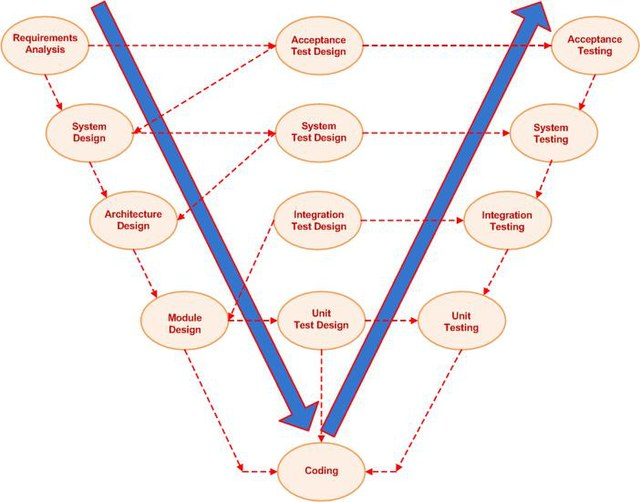
\includegraphics[scale=0.5]{img/V-model.JPG}
        \caption{Le frecce blu rappresentano il \emph{tempo}, mentre quelle tratteggiate le \emph{dipendenze}}
    \end{figure}
\end{center}

Questo modello evidenzia come sia possibile progettare i \textcolor{cyan}{test}
durante le fasi di sviluppo (quelle a sinistra, prima della fase di \emph{coding}). Mentre sulla destra
sono presenti i test veri e propri che devono verificare e convalidare l'attività in corrispondenza sulla sinistra.

\paragraph{\textcolor{ForestGreen}{Standard SQA}}
Questo modello è uno degli standard \emph{SQA} (Software Quality Assurance), usato
per descrivere le attività di test durante il processo di sviluppo.

\subsection{Modelli Iterativi}

\subsubsection{Rapid Prototyping}

L'obbiettivo è quello di costruire rapidamente un prototipo del software per permettere al committente di sperimentarlo.

Questo modello diventa utile quando i requisiti non sono chiari, quindi ogni prototipo aiuterà il cliente a descriverli meglio.

\begin{center}
    \begin{tikzpicture}[main/.style={rectangle, draw}]
        \node[main] (1) {Analisi Preliminare};
        \node[main] (2) [below right=1cm and 0.1cm of 1] {Analisi e Progettazione};
        \node[main] (3) [below right=1cm and 0.1cm of 2] {\begin{tabular}{c}Realizzazione del \\ prototipo (usa e getta)\end{tabular}};
        \draw[thick, ->] (1) -| (2);
        \draw[thick, ->] (2) -| (3);
        \draw[thick, ->] (3) -| (2);
    \end{tikzpicture}
\end{center}

\subsubsection{Modello Incrementale}